\documentclass[11pt]{article}
\usepackage[a4paper, margin=2.5cm]{geometry}

% Slovenščina in kodiranje
\usepackage[slovene]{babel}
\usepackage[utf8]{inputenc}
\usepackage[T1]{fontenc}

\usepackage{graphicx}
\usepackage{amsmath}
\usepackage{amssymb}
\usepackage{amsthm}

% Okolji definicija in izrek
\theoremstyle{definition}
\newtheorem{definicija}{Definicija}

\theoremstyle{plain}
\newtheorem{izrek}{Izrek}

% Pisani F
\newcommand{\f}{\mathcal{F}}

\title{Brownovo gibanje}
\author{Matej Rojec}
\date{}

\begin{document}

\maketitle

Brownovo gibanje (več v~\cite{karatzas1991brownian}) je intuitivno slučajen proces,
ki predstavlja naključno gibanje delcev v mediju.

\begin{figure}[!ht]
   \centering
   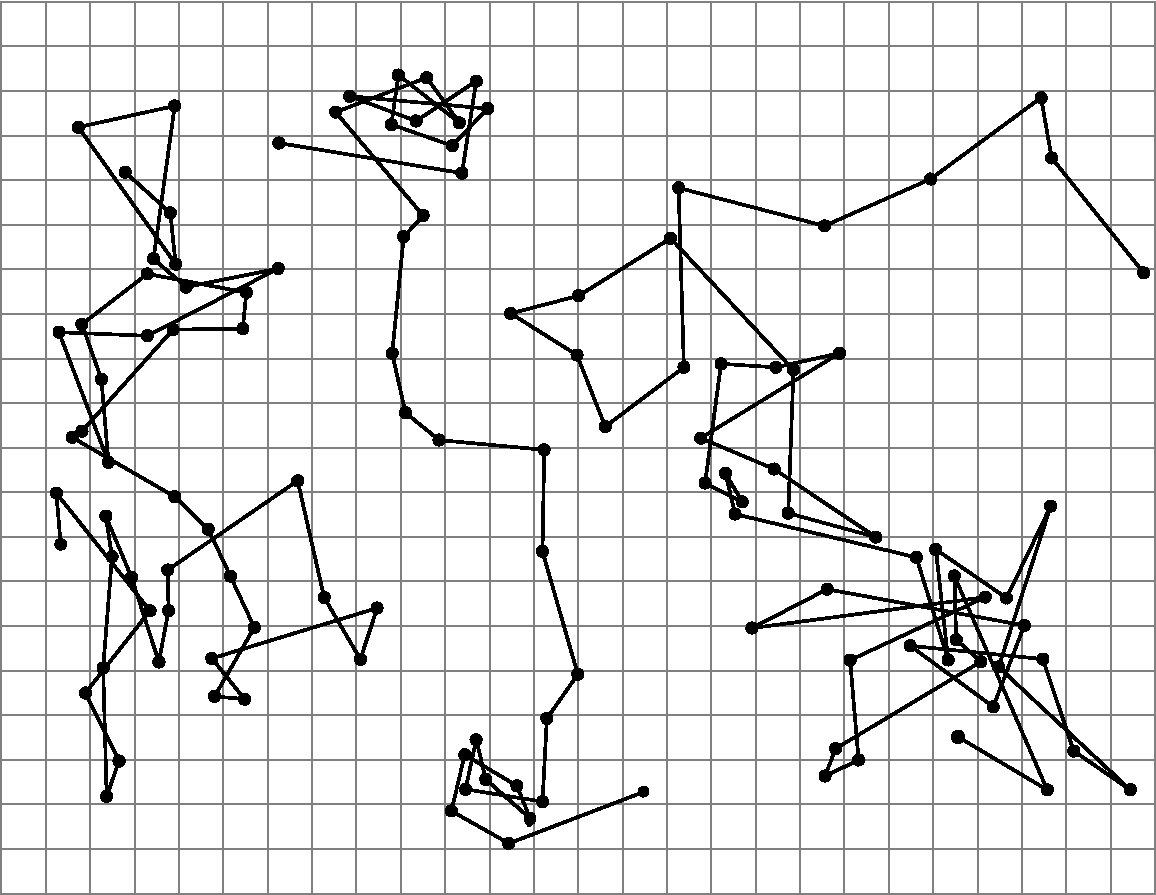
\includegraphics[scale=0.3]{PerrinPlot2.pdf}
   \caption{Reprodukcija slike iz Jean Baptiste Perrin, \emph{Mouvement brownien et réalité moléculaire}, Ann. de Chimie et de Physique (VIII) 18, 5-114, 1909}
\end{figure}

\begin{definicija}
   \emph{Standardno Brownovo gibanje} \(\{B_t\}_{t \geq 0}\) je slučajen proces z naslednjimi lastnostmi:
   \begin{enumerate}
      \item \(B_0 = 0\).
      \item Prirastki \(B_{t_n} - B_{t_{n-1}}, B_{t_{n-1}} - B_{t_{n-2}}, \ldots, B_{t_2} - B_{t_1}, B_{t_1} - B_{t_0}\) so neodvisne slučajne spremenljivke, za vsak \(t_0 \leq t_1 \leq \cdots \leq t_{n-1} \leq t_n\).
      \item Za vsak \(t \geq 0\) in \(h > 0\) velja \(B_{t+h} - B_t \sim \mathcal{N}(0, h)\).
      \item Funkcija \(t \mapsto B_t\) je zvezna skoraj gotovo.
   \end{enumerate}
\end{definicija}

Preden zapišemo izrek, definirajmo še pojem časa ustavljanja.

\begin{definicija}
   Slučajna spremenljivka \(\tau\) na verjetnostnem prostoru \((\Omega, \f, P)\) z vrednostmi v \(\mathbb{R}^+\)
   je \emph{čas ustavljanja} glede na filtracijo \((\f_t)_{t \in T}\), če velja: \(\forall t \in T : \{\tau \leq t\} \in \f_t\).
\end{definicija}

Zdaj lahko zapišemo izrek~\ref{thm:stopped_brownian}.

\begin{izrek}
   \label{thm:stopped_brownian}
   Naj bo \(\{B_t\}_{t \geq 0}\) (standardno) Brownovo gibanje, \(\tau\) čas ustavljanja glede na
   \((\f_t)_{t \geq 0}\) in naj velja \(P[\tau < \infty] = 1\).
   Potem je tudi proces:
   \[
      \hat{B} := \{B_{\tau+t} - B_\tau \mid t \geq 0\}
   \]
   (standardno) Brownovo gibanje in neodvisen od \(\f_\tau\).
\end{izrek}

\bibliographystyle{plain}
\bibliography{knjiga}

\end{document}
